% Homework template created by Jonathan Wheeler
% for use at Stanford University.
% Edited by Lucas Saldyt
%
% Adapted from a jhwhw.cls file I found on
% github.
%
% In sublime, use Cmd-L, backspace to 
% clear auxiliary files 

\documentclass[notitlepage]{homework}

\usepackage{amssymb}
\usepackage{amsmath}
\usepackage[parfill]{parskip}
\usepackage{minted}
\usepackage{graphicx}
\usepackage{tikz}
\usepackage{pgfplots}
\usepackage[euler]{textgreek}
\usepackage{multicol}
\usepackage{siunitx}
\usepackage{subcaption}

\pgfplotsset{compat=1.13}
\usetikzlibrary{decorations.pathmorphing,shapes}
\usepgfplotslibrary{fillbetween}
\usetikzlibrary{calc}

\newcommand{\AssignmentName}{TITLE}

\author{Lucas Saldyt} %TODO
\title{\AssignmentName}


\begin{document}
% Used in syntax highlighting
\definecolor{bg}{rgb}{0.95,0.95,0.95}

\begin{titlepage}
	\begin{center}
		{\Large \AssignmentName}
		
		\bigskip

		\begin{tabular}{rl}
			ID: & 12345678 \\ % TODO
            Name: & Lucas Saldyt (lsaldyt@asu.edu) \\ % TODO
			Collaborators: & $\varnothing$
		\end{tabular}

		\bigskip

	\end{center}

	\toccontents

	\vfill

\end{titlepage}

% TODO
\problem{Quadratic Values}

\begin{enumerate}
    \item Plot the equation $y = x^2 - 1$ for $-5 < x < 5$
    \item What is the minimum?
\end{enumerate}

\solution

\part 

Using the following python code:

\inputminted{python}{code/p1.py}

\begin{center}
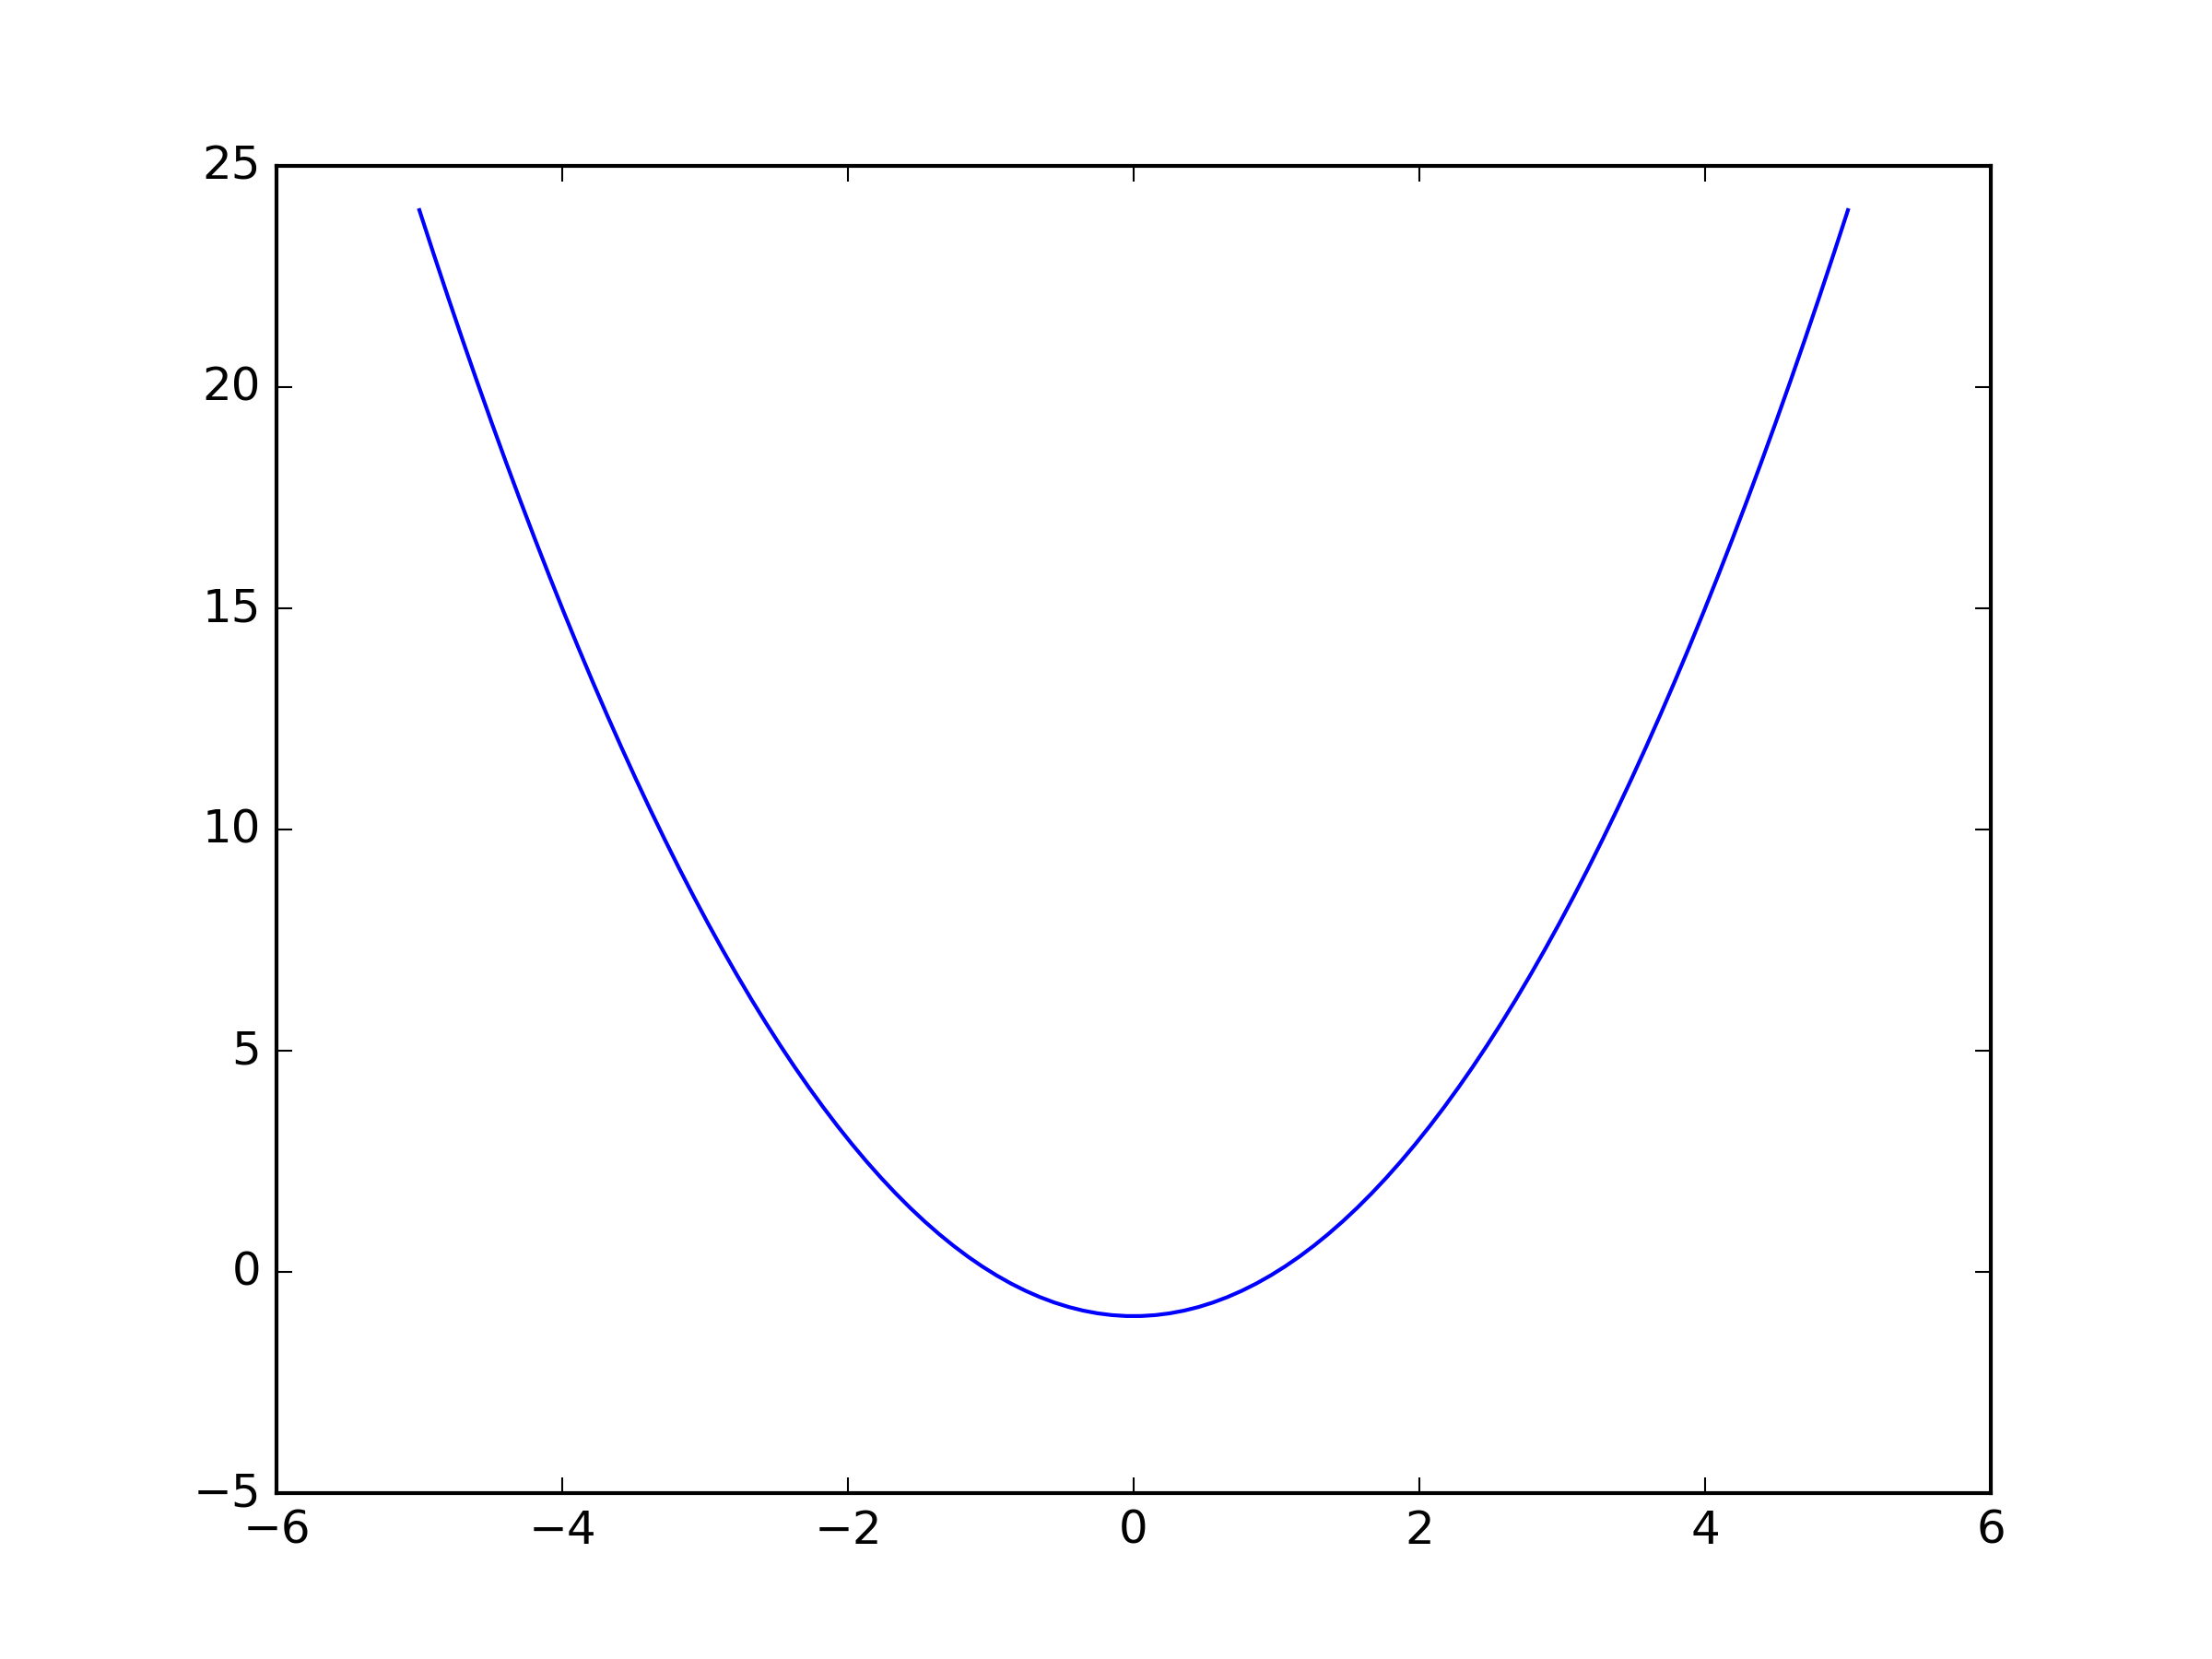
\includegraphics[width=.5\textwidth]{images/p1.png}
\end{center}

\part

The minimum is found by looking for zeros in the derivative.

$$ \frac{\partial y}{\partial x} = 2x$$

This has a zero at \fbox{$x = 0$}.

\problem{Data Analysis}

\begin{enumerate}
  \item Using the data in sample.csv, find the line of best fit through the data.
  \item Plot this data with the line.
\end{enumerate}

\solution

\part 

$m = 0.5$, $b = 1.5$

\part

\begin{center}
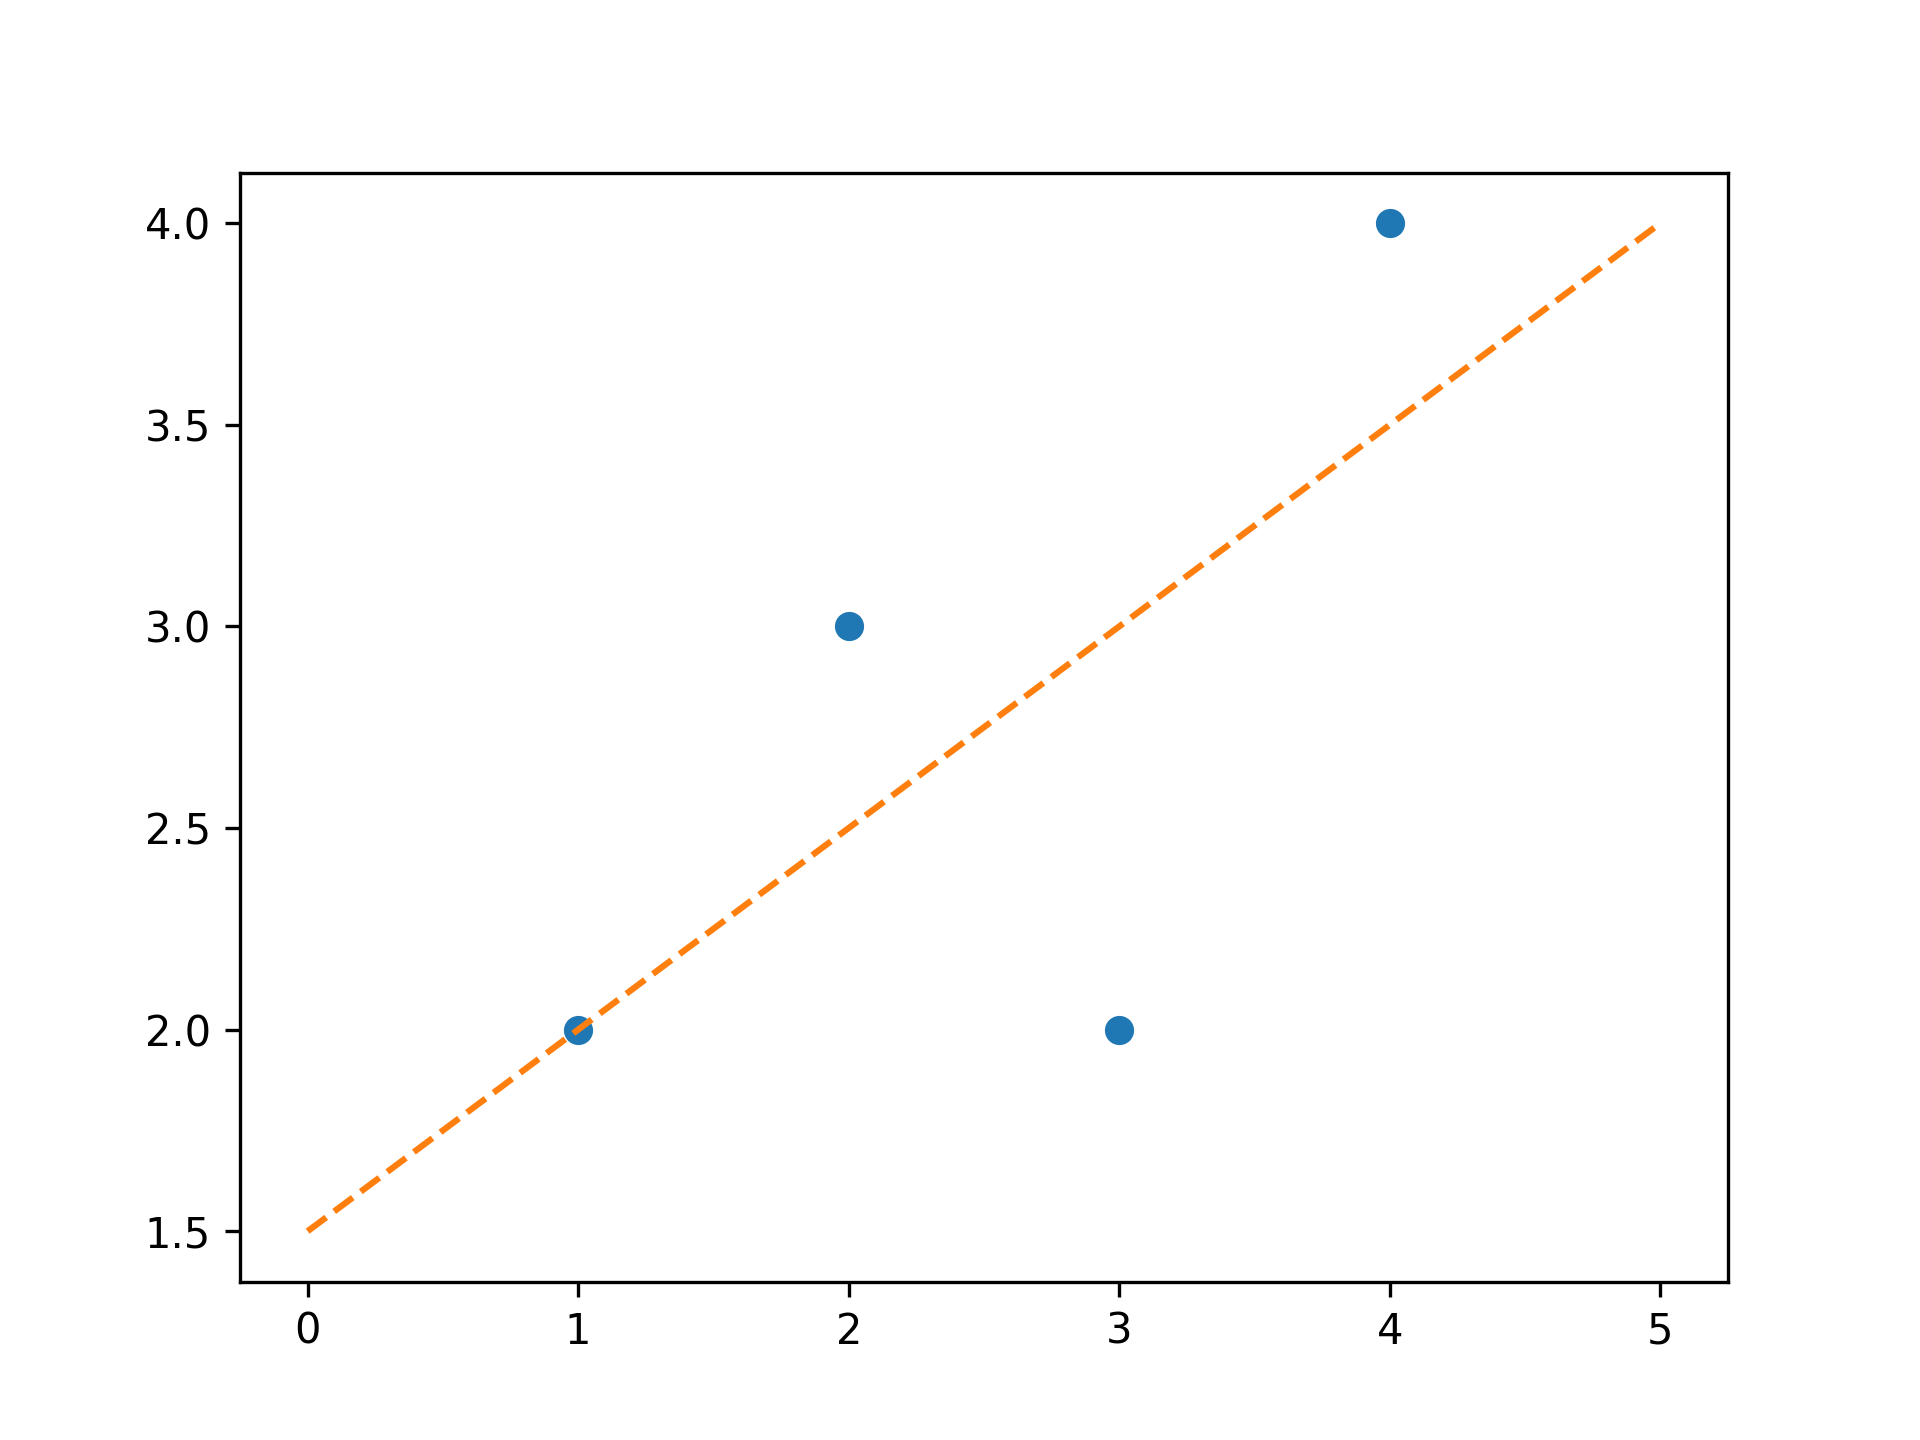
\includegraphics[width=.5\columnwidth]{images/p2.png}
\end{center}


\end{document}
